\chapter{Lagrangianos, campos y procesos locales de partículas}

Los campos bosónicos, los campos fermiónicos y el campo electromagnético obedecen ecuaciones de tipo ondulatorio. Estas ecuaciones involucran los propios campos y sus derivadas espaciales y temporales. Se podría enumerar una ecuación de movimiento independiente para cada campo, pero un lagrangiano reúne todo el sistema en una sola expresión compacta. Al aplicar a esta expresión la regla de Euler--Lagrange se obtienen de una vez las ecuaciones de todos los campos.

Esta construcción está estrechamente relacionada con la acción estacionaria. Aquí la tarea inmediata es más concreta: identificar de qué depende un lagrangiano de campo, utilizarlo para obtener algunas ecuaciones clásicas y reinterpretar después esas mismas expresiones de campo en términos cuánticos. En la teoría cuántica, el lagrangiano rige el movimiento y la interacción de las partículas y, en última instancia, las amplitudes y secciones eficaces de las colisiones.

\section{Una expresión compacta para las ecuaciones de campo}

Para un campo escalar, la densidad lagrangiana depende del campo y de sus primeras derivadas,
\begin{equation}
\mathcal L
=
\mathcal L\!\left(\phi,\partial_t\phi,\partial_x\phi,\ldots\right)
=
\mathcal L\!\left(\phi,\partial_\mu\phi\right).
\end{equation}
Al calcular, suele ser más útil escribir explícitamente la lista de derivadas temporales y espaciales; la notación \(\partial_\mu\phi\) agrupa esa misma lista en forma relativista.

\begin{figure}[htbp]
\centering
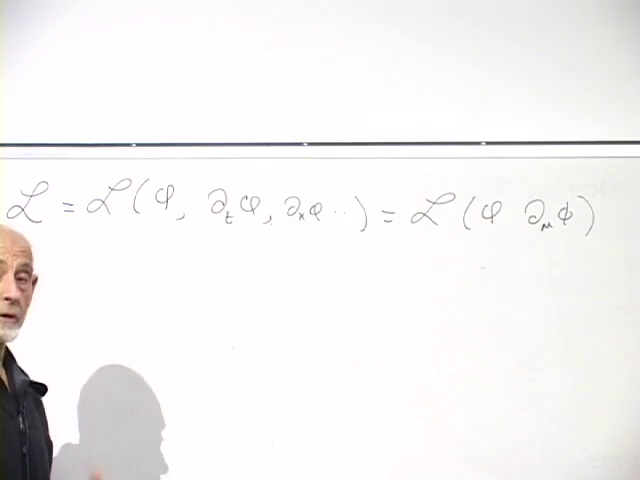
\includegraphics[width=0.82\textwidth]{lecture_09_figure_03.png}
\caption{Dependencia de un lagrangiano de campo escalar respecto del campo y de sus derivadas espaciotemporales.}
\lectureframe{00:03:56}
\end{figure}

La ecuación de Euler--Lagrange para campos es
\begin{equation}
\frac{\partial}{\partial t}
\frac{\partial\mathcal L}{\partial\dot\phi}
+
\frac{\partial}{\partial x}
\frac{\partial\mathcal L}{\partial\phi_x}
+
\frac{\partial}{\partial y}
\frac{\partial\mathcal L}{\partial\phi_y}
+
\frac{\partial}{\partial z}
\frac{\partial\mathcal L}{\partial\phi_z}
=
\frac{\partial\mathcal L}{\partial\phi},
\end{equation}
donde
\begin{equation}
\dot\phi=\frac{\partial\phi}{\partial t},
\qquad
\phi_x=\frac{\partial\phi}{\partial x},
\qquad
\phi_y=\frac{\partial\phi}{\partial y},
\qquad
\phi_z=\frac{\partial\phi}{\partial z}.
\end{equation}
Si \(\mathcal L\) contiene varios campos, esta regla se aplica una vez a cada uno. El resultado es el sistema de ecuaciones de movimiento.

El ejemplo escalar más sencillo es
\begin{equation}
\begin{split}
\mathcal L
&=
\frac12\dot\phi^2
-\frac12\phi_x^2
-\frac12\phi_y^2
-\frac12\phi_z^2
-V(\phi)
\\
&=
\frac12\dot\phi^2-\frac12(\boldsymbol\nabla\phi)^2-V(\phi).
\end{split}
\end{equation}
Los términos de derivadas espaciales tienen signo opuesto al término de la derivada temporal. Al derivar término a término se obtiene
\begin{align}
\frac{\partial\mathcal L}{\partial\dot\phi}&=\dot\phi,
&
\frac{\partial\mathcal L}{\partial\phi_i}&=-\phi_i,
&
\frac{\partial\mathcal L}{\partial\phi}&=-V'(\phi),
\end{align}
y, por tanto,
\begin{equation}
\ddot\phi-\nabla^2\phi=-V'(\phi).
\end{equation}

\begin{figure}[htbp]
\centering
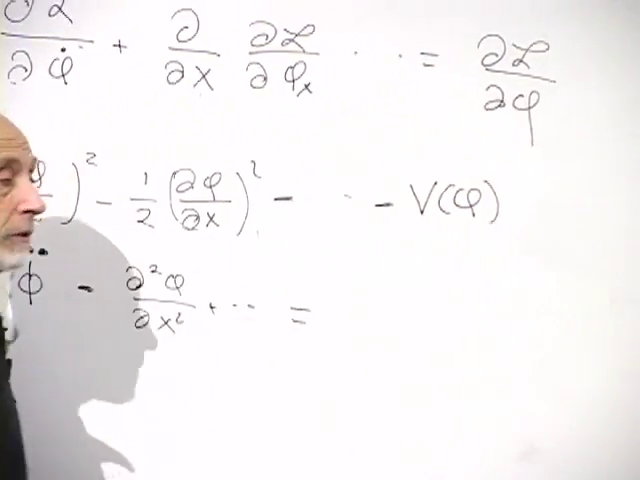
\includegraphics[width=0.74\textwidth]{lecture_09_figure_04.png}
\caption{Ecuación de Euler--Lagrange, lagrangiano de campo escalar y ecuación de campo generada por \(V(\phi)\).}
\lectureframe{00:08:23}
\end{figure}

Esta es la ecuación que genera el lagrangiano escalar.\editorialnote{El fotograma conservado está recortado por el borde izquierdo; la continuación mostrada queda determinada por la derivación oral inmediatamente anterior y posterior.}

Aquí \(V(\phi)\) es la densidad de energía potencial del campo. Una contribución constante a \(V\) no afecta esta ecuación porque su derivada se anula. Un potencial lineal es algebraicamente posible, pero no está acotado inferiormente: la energía del campo puede tender a menos infinito. Por tanto, el primer ejemplo estable es
\begin{equation}
V(\phi)=\frac12m^2\phi^2,
\qquad
V'(\phi)=m^2\phi,
\end{equation}
que da lugar a
\begin{equation}
\ddot\phi-\nabla^2\phi=-m^2\phi.
\end{equation}

Para mostrar el significado de \(m\), se sustituye una onda plana,
\begin{equation}
\phi(\mathbf x,t)=\phi_0e^{i\omega t-i\mathbf k\cdot\mathbf x}.
\end{equation}
Entonces,
\begin{equation}
\ddot\phi=-\omega^2\phi,
\qquad
\nabla^2\phi=-\mathbf k^2\phi,
\end{equation}
de modo que la ecuación de onda se convierte en
\begin{equation}
-\omega^2\phi+\mathbf k^2\phi=-m^2\phi.
\end{equation}
Tras cancelar \(\phi\),
\begin{equation}
\omega^2=\mathbf k^2+m^2.
\end{equation}
En unidades en las que \(\hbar=c=1\), la frecuencia es la energía y el número de onda es el momento. Por tanto,
\begin{equation}
E^2=\mathbf p^2+m^2,
\end{equation}
o, al restituir las potencias de \(c\), \(E^2=\mathbf p^2c^2+m^2c^4\). El parámetro \(m\) es la masa de un cuanto del campo.

La invariancia relativista puede imponerse directamente a la expresión compacta. Si \(\mathcal L\) es un escalar de Lorentz, sus ecuaciones de movimiento son invariantes de Lorentz. El signo relativo entre las derivadas temporales y espaciales es el conocido signo espaciotemporal de la relatividad especial.

\section{No linealidad y campos clásicos acoplados}

Las potencias superiores de un campo introducen un comportamiento nuevo. Si
\begin{equation}
V(\phi)=\frac12m^2\phi^2+g\phi^3,
\end{equation}
entonces
\begin{equation}
\ddot\phi-\nabla^2\phi=-m^2\phi-3g\phi^2.
\end{equation}
Los términos cuadráticos del lagrangiano dan ecuaciones lineales en el campo. Los términos cúbicos y de orden superior dan ecuaciones no lineales.

La diferencia se aprecia en el movimiento de los paquetes de onda. Para una ecuación lineal, se pueden sumar un paquete que se propaga hacia la derecha y otro que se propaga hacia la izquierda para obtener otra solución. Se superponen e interfieren durante un tiempo, luego se atraviesan y emergen con sus formas originales. Cuando hay términos no lineales, los paquetes se influyen mutuamente. Pueden dispersarse, deformarse o descomponerse en ondas más complejas. La interferencia transitoria de las ondas lineales no es una interacción; un cambio duradero en los paquetes indica no linealidad.

El mismo patrón aparece con dos campos escalares. Sean
\begin{align}
\mathcal L
&=
\frac12(\partial_\mu\phi)(\partial^\mu\phi)
+\frac12(\partial_\mu\rho)(\partial^\mu\rho)
-V(\phi,\rho),
\\
V(\phi,\rho)
&=
\frac12m^2\phi^2+\frac12M^2\rho^2+\rho\phi^2.
\end{align}
Sin el último término, las dos ecuaciones son independientes:
\begin{equation}
\ddot\phi-\nabla^2\phi=-m^2\phi,
\qquad
\ddot\rho-\nabla^2\rho=-M^2\rho.
\end{equation}
Describen cuantos de dos especies, con masas \(m\) y \(M\). Al incluir el término mixto,
\begin{align}
\ddot\phi-\nabla^2\phi&=-m^2\phi-2\rho\phi,
\\
\ddot\rho-\nabla^2\rho&=-M^2\rho-\phi^2.
\end{align}
cada ecuación contiene ahora el otro campo. Las ecuaciones están acopladas y son no lineales: un paquete \(\phi\) se dispersa al interactuar con un paquete \(\rho\), y viceversa. Los términos con derivadas determinan la relación entre energía--momento, los términos cuadráticos sin derivadas fijan las masas y el término mixto de orden superior codifica la interacción. Este es el patrón clásico básico.

\section{Campos de Dirac y acoplamiento escalar}

Para un campo de Dirac, la ecuación es de primer orden en el tiempo. En una notación abreviada unidimensional, entendiendo que se extiende a tres dimensiones espaciales, la estructura de sus términos es
\begin{equation}
i\dot\Psi
\simeq
i\alpha\frac{\partial\Psi}{\partial x}+m\beta\Psi,
\qquad
i\boldsymbol\alpha\cdot\boldsymbol\nabla\Psi
=i\sum_i\alpha_i\frac{\partial\Psi}{\partial x_i}.
\end{equation}
Las matrices \(\alpha_i\) y \(\beta\) actúan sobre las componentes de \(\Psi\). Un lagrangiano correspondiente contiene un término lineal en \(\partial_t\Psi\), un término bilineal con derivadas espaciales que involucra \(\alpha_i\) y el término bilineal de masa \(m\Psi^\dagger\beta\Psi\). Aquí solo hace falta este hecho estructural.\editorialnote{En la fuente se deja explícitamente sin resolver si los signos, los paréntesis y la posición de \(i\) son correctos en el lagrangiano de Dirac propuesto. No se infiere de él ninguna fórmula exacta que dependa de una convención.}

\begin{figure}[htbp]
\centering
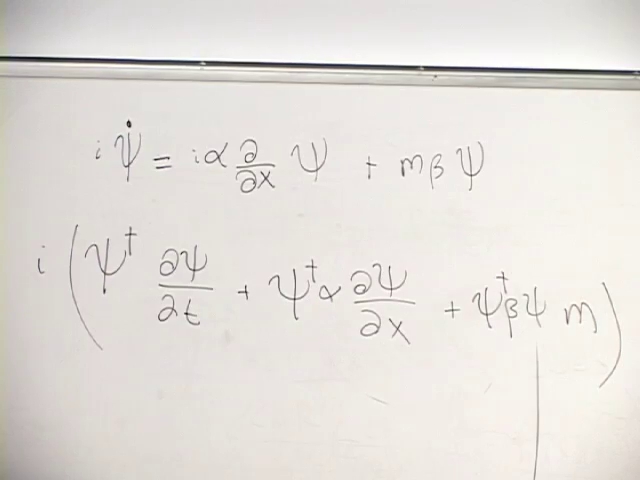
\includegraphics[width=0.76\textwidth]{lecture_09_figure_05.png}
\caption{Términos de derivada temporal, derivada espacial y masa en el análisis del campo de Dirac.}
\lectureframe{00:25:37}
\end{figure}

\begin{classroomqa}
\lecturetimestamp{00:26:37}
\audiencequestion{¿Está correctamente colocado el paréntesis en el lagrangiano de Dirac propuesto, de modo que \(i\) multiplique toda la expresión?}
\lecturerresponse{Aquí no se fija con seguridad la posición del paréntesis, y no hace falta para el punto estructural: existe un lagrangiano que genera la ecuación de Dirac.}
\end{classroomqa}

Añadamos ahora un campo escalar \(\phi\). El producto ingenuo \(\Psi^\dagger\Psi\,\phi\) no es un escalar de Lorentz. Al insertar la misma matriz de Dirac que aparece en el término de masa se obtiene
\begin{equation}
\mathcal L_{\mathrm{int}}
\propto
\Psi^\dagger\beta\Psi\,\phi.
\end{equation}
Equivalentemente, \(\Psi^\dagger\beta\Psi\) es el término bilineal escalar de Dirac. Al variar el lagrangiano completo, se añade a la ecuación de Dirac un término proporcional a \(\phi\) y a la ecuación escalar una fuente proporcional a \(\Psi^\dagger\beta\Psi\). Los dos campos se dispersan mutuamente.

\begin{classroomqa}
\lecturetimestamp{00:28:03}
\audiencequestion{¿Es la \(\beta\) que se inserta en la interacción escalar--fermiónica la misma \(\beta\) que aparece en el término de masa de Dirac?}
\lecturerresponse{Sí. Es la misma matriz de Dirac.}
\end{classroomqa}

La comparación
\begin{equation}
m\Psi^\dagger\beta\Psi
\qquad\hbox{and}\qquad
\Psi^\dagger\beta\Psi\,\phi
\end{equation}
hace que el acoplamiento parezca un parámetro de masa sustituido por un campo escalar. Esta observación reaparecerá cuando, hacia el final, se considere un campo cuyo valor de vacío no es nulo.

Hasta ahora la interpretación ha sido clásica: los paquetes de onda se dispersan unos con otros. El mismo álgebra adquiere un significado más preciso en términos de partículas cuando los campos pasan a ser operadores.

\section{Qué hacen las potencias de los campos cuánticos}

Un campo cuántico escalar real contiene operadores de creación y aniquilación. Esquemáticamente,
\begin{equation}
\phi(x)\sim A^+(x)+A^-(x),
\end{equation}
donde \(A^+\) crea un cuanto y \(A^-\) lo aniquila. Por consiguiente, \(\phi^3(x)\) contiene cuatro tipos de procesos locales:
\begin{equation}
\phi^3
\sim
(A^+)^3+(A^+)^2A^-+A^+(A^-)^2+(A^-)^3,
\end{equation}
en esta interpretación esquemática se omiten los detalles de ordenamiento y los coeficientes numéricos. Los cambios en el número de partículas son
\begin{equation}
3\longrightarrow0,
\qquad
0\longrightarrow3,
\qquad
2\longrightarrow1,
\qquad
1\longrightarrow2.
\end{equation}
Los tres factores de campo actúan en el mismo punto \(x\). Así, un solo término cúbico incluye la aniquilación de tres partículas, la creación de tres partículas, la fusión de dos cuantos en uno y la división de uno en dos. En una amplitud física, la conservación de la energía--momento puede descartar después algunas de estas interpretaciones locales, pero todas están presentes en el propio producto de operadores.

Los términos cuadráticos libres cumplen otra función. Primero, omitamos la normalización de la diferencia entre los puntos vecinos \(x\) y \(x'\):
\begin{equation}
\partial_x\phi
\ \propto\
\phi(x)-\phi(x').
\end{equation}
Al elevar al cuadrado y desarrollar se obtiene la estructura de términos
\begin{align}
\frac12(\partial_x\phi)^2
&\ \propto\
\frac12\bigl[\phi(x)-\phi(x')\bigr]^2
\\
&=
\frac12\phi(x)^2
+\frac12\phi(x')^2
-\phi(x)\phi(x').
\end{align}
Cada cuadrado en un mismo punto admite varias interpretaciones en términos de operadores: puede crear dos cuantos, aniquilar dos o aniquilar y volver a crear uno en ese mismo punto. Esos términos no transportan una partícula. El término cruzado puede aniquilar un cuanto en \(x'\) y crearlo en \(x\), o al revés. Por tanto, actúa como un término de salto entre puntos vecinos. Los factores repetidos llevan una partícula de \(x\) a \(x'\), luego a \(x''\) y así sucesivamente. Los términos cuadráticos con derivadas rigen la propagación libre; los términos cúbicos y de orden superior dispersan, crean y aniquilan partículas.

\begin{classroomqa}
\lecturetimestamp{00:36:07}
\audiencequestion{¿Debe incluir la representación de la derivada por diferencias finitas la separación \(x-x'\)?}
\lecturerresponse{Sí. Si se llama \(L\) a la separación, al elevar la diferencia al cuadrado aparece el factor \(L^{-2}\). Ese factor numérico cambia el coeficiente, pero no la interpretación como salto.}
\end{classroomqa}

Al restituir la separación se obtiene
\begin{align}
\frac12(\partial_x\phi)^2
&\longrightarrow
\frac{1}{2L^2}\bigl[\phi(x)-\phi(x')\bigr]^2
\\
&=
\frac{1}{2L^2}\phi(x)^2
+\frac{1}{2L^2}\phi(x')^2
-\frac{1}{L^2}\phi(x)\phi(x').
\end{align}

El término de masa también es cuadrático, pero no contiene derivadas:
\begin{equation}
\frac12m^2\phi(x)^2.
\end{equation}
Su interpretación para una partícula es la de un cuanto que llega, es absorbido y vuelve a emitirse en el mismo punto. No desplaza el cuanto; pondera su presencia allí o, en ese sentido, la cuenta. El mismo cuadrado de operadores también admite las interpretaciones de creación de dos cuantos y aniquilación de dos. Así pues, para el movimiento la diferencia pertinente está entre un término cruzado que conecta puntos vecinos y una inserción de masa que actúa en un solo punto.

\section{El vértice local de la electrodinámica cuántica}

Estos esquemas elementales de procesos entre partículas son el punto de partida de los diagramas de Feynman. El ejemplo central es la electrodinámica cuántica, la teoría de los electrones, los positrones y los fotones.

La ecuación de Dirac tiene modos de energía positiva y negativa. En el lenguaje antiguo, \(\Psi\) contiene operadores de aniquilación para ambos tipos de modo, mientras que \(\Psi^\dagger\) contiene los operadores de creación correspondientes. La eliminación de un electrón de energía negativa se reinterpreta como la creación de un positrón de energía positiva. Tras ese cambio de etiquetas, la descomposición esquemática útil es
\begin{align}
\Psi
&\sim
C^-_{e^-}+C^+_{e^+},
\\
\Psi^\dagger
&\sim
C^+_{e^-}+C^-_{e^+}.
\end{align}
Así, \(\Psi\) aniquila un electrón o crea un positrón, mientras que \(\Psi^\dagger\) crea un electrón o aniquila un positrón. Esta abreviatura no implica ningún factor de normalización, etiqueta de espín ni integral sobre el momento.

La interacción de la electrodinámica cuántica acopla la corriente de Dirac al potencial vector electromagnético. En la notación por componentes que se usa aquí, su estructura es
\begin{equation}
\mathcal L_{\mathrm{QED,int}}
\sim
e\left(
\Psi^\dagger\Psi\,A_0
+
\Psi^\dagger\boldsymbol{\alpha}\Psi\mathbin{\boldsymbol{\cdot}}\mathbf A
\right),
\end{equation}
donde
\begin{equation}
J^0=\Psi^\dagger\Psi,
\qquad
\mathbf J=\Psi^\dagger\boldsymbol{\alpha}\Psi.
\end{equation}
El símbolo \(\sim\) es importante: el signo relativo entre los términos temporal y espacial depende de las convenciones para la métrica y el potencial vector. La afirmación invariante es que la corriente de cuatro componentes se contrae con el potencial de cuatro componentes.\editorialnote{La fuente fija las componentes temporales y espaciales de la corriente, pero no especifica una convención métrica para la contracción de componentes.}

El propio campo de fotones \(A_\mu\) contiene operadores de creación y aniquilación de fotones. Su carácter vectorial también codifica la polarización del fotón---una pequeña ``marca'' direccional además de su momento.

\begin{classroomqa}
\lecturetimestamp{00:44:28}
\audiencequestion{¿Cómo puede la interacción ser un escalar si \(A_\mu\) es un vector y el factor fermiónico parece, a primera vista, un escalar?}
\lecturerresponse{Los fermiones también aportan un vector de cuatro componentes: \(\Psi^\dagger\Psi\) es su componente temporal y \(\Psi^\dagger\boldsymbol\alpha\Psi\) su componente espacial. Al contraer esa corriente con \(A_\mu\) se obtiene un escalar.}
\end{classroomqa}

Al multiplicar el contenido de operadores de \(\Psi^\dagger\), \(\Psi\) y \(A_\mu\) se obtienen cuatro interpretaciones conocidas de un mismo vértice local:
\begin{enumerate}
\item un electrón emite un fotón;
\item un electrón absorbe un fotón;
\item un electrón y un positrón se aniquilan y producen un fotón;
\item un fotón crea un par electrón--positrón.
\end{enumerate}
En la primera interpretación, \(\Psi\) aniquila el electrón entrante, \(\Psi^\dagger\) crea el electrón saliente y el campo de fotones crea el fotón. Si se elige la parte de aniquilación del fotón, se obtiene la absorción. Al elegir las partes correspondientes al positrón, se obtiene la aniquilación o la creación de pares. Un término local contiene toda esta familia.

En un diagrama de flujo fermiónico, la flecha de una línea de positrón apunta en sentido opuesto a la dirección de propagación del positrón. Con esta convención, la flecha fermiónica atraviesa de forma continua todos los vértices permitidos de la electrodinámica cuántica. Las cuatro interpretaciones difieren en que las líneas externas se trasladan entre los lados entrante y saliente; la línea de flujo fermiónico no se interrumpe.

Todas estas interpretaciones llevan el mismo coeficiente \(e\), la carga eléctrica en la convención microscópica empleada. Este coeficiente es la carga eléctrica \(e\), no la constante de estructura fina, aunque ambas están estrechamente relacionadas. La amplitud del vértice es proporcional a \(e\); una vez incluidos todos los factores cinemáticos y de normalización, la escala correspondiente de probabilidad es proporcional a \(e^2\).

\begin{classroomqa}
\lecturetimestamp{00:49:44}
\audiencequestion{¿La interpretación en que un fotón da lugar a un electrón--positrón lleva el mismo coeficiente que las otras interpretaciones del vértice?}
\lecturerresponse{Sí. Lleva el mismo coeficiente de carga eléctrica \(e\).}
\end{classroomqa}

\begin{classroomqa}
\lecturetimestamp{00:49:59}
\audiencequestion{¿No debería haber un factor de escala, dado que una probabilidad no tiene unidades?}
\lecturerresponse{En la convención microscópica natural que se emplea, la carga \(e\) es adimensional. Esta fija la escala de la amplitud y su cuadrado fija la escala de la probabilidad.}
\end{classroomqa}

Consideremos el caso concreto de un electrón que choca contra una pared y se detiene bruscamente. Existe cierta probabilidad de que se emitan energía y momento en forma de fotón. El factor electromagnético elemental en la amplitud de esa radiación es \(e\), por lo que la escala de probabilidad contiene \(e^2\). Esta afirmación aísla el factor de acoplamiento; la probabilidad real también depende del estado del electrón y de la cinemática.

\begin{figure}[htbp]
\centering
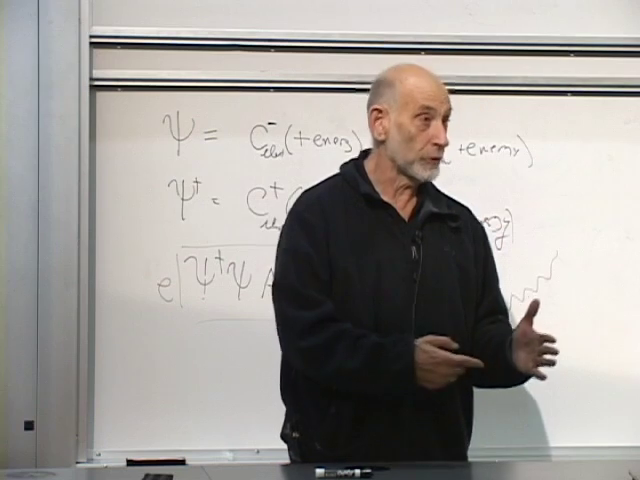
\includegraphics[width=0.78\textwidth]{lecture_09_figure_06.png}
\caption{Contenido de operadores de electrones y positrones en \(\Psi\) y \(\Psi^\dagger\), con un esquema de interacción electrón--fotón.}
\lectureframe{00:50:39}
\end{figure}

\begin{classroomqa}
\lecturetimestamp{00:51:15}
\audiencequestion{¿Tiene unidades la carga eléctrica?}
\lecturerresponse{No en la convención microscópica natural que se usa aquí. La carga macroscópica suele expresarse en culombios, pero la teoría de partículas mide la carga respecto de una unidad elemental elegida. En unidades de Planck u otras unidades naturales, las magnitudes se expresan como números puros.}
\end{classroomqa}

La diferencia se debe a las convenciones y a las escalas. Los culombios son prácticos para describir la corriente en los cables; un acoplamiento adimensional es práctico para las amplitudes microscópicas.\editorialnote{Una breve pregunta de 00:52:37--00:53:15 sobre la ``agrupación'' de los términos que llevan carga está muy dañada y no dio lugar a ninguna construcción definida.}

Los tres campos de la interacción elemental de la electrodinámica cuántica se evalúan en un mismo punto espaciotemporal. Al vértice mismo no se le asigna ningún retardo temporal interno.

\begin{classroomqa}
\lecturetimestamp{00:53:19}
\audiencequestion{¿Son simultáneas la absorción y reemisión del electrón y la emisión del fotón, o la ecuación incorpora un retardo?}
\lecturerresponse{En el vértice elemental, todos los operadores se evalúan en el mismo punto espaciotemporal. Por tanto, el proceso básico no tiene ningún retardo entre esos actos.}
\end{classroomqa}

\begin{classroomqa}
\lecturetimestamp{00:53:57}
\audiencequestion{¿Debe conservarse cada cantidad conservada por separado?}
\lecturerresponse{Sí. La carga eléctrica es una de las cantidades que deben conservarse por separado.}
\end{classroomqa}

La conservación de la carga se aprecia tanto en el diagrama como en el álgebra. Un proceso que transformara un electrón entrante en un positrón saliente invertiría la carga y no sería un vértice permitido de la electrodinámica cuántica. Si el tiempo se representa hacia arriba, la flecha del electrón apunta hacia arriba en la dirección del tiempo y la del positrón hacia abajo; en el vértice permitido, la flecha fermiónica siempre lo atraviesa de un lado al otro. Algebraicamente, la interacción contiene un \(\Psi\) y un \(\Psi^\dagger\). El primero aumenta la carga en una unidad cuando aniquila un electrón o crea un positrón, y el segundo la reduce en una unidad. Sus efectos se cancelan.

\begin{classroomqa}
\lecturetimestamp{00:56:05}
\audiencequestion{¿Es la expresión recuadrada de electrón--fotón todo el lagrangiano de la electrodinámica cuántica?}
\lecturerresponse{No. Es el término de interacción. No se han escrito los términos cuadráticos del fotón libre ni los términos cuadráticos de Dirac, que rigen la propagación.}
\end{classroomqa}

\begin{classroomqa}
\lecturetimestamp{00:56:35}
\audiencequestion{¿Se deduce un lagrangiano clásico mientras que el lagrangiano cuántico se propone y se pone a prueba? ¿Se mantiene en mecánica cuántica la estructura de energía cinética menos energía potencial?}
\lecturerresponse{Se mantiene el patrón de energía cinética menos energía potencial: las derivadas temporales aportan la forma cinética, los gradientes espaciales la generalizan y los términos de campo sin derivadas aportan la forma potencial. El lagrangiano cuántico es la descripción más fundamental. En un estado con muchísimos cuantos, el mismo lagrangiano produce las ecuaciones de onda clásicas. Los lagrangianos candidatos se proponen a partir de principios físicos y teorías más profundas, y luego se confirman o se descartan mediante experimentos de colisión.}
\end{classroomqa}

El límite de ocupación elevada explica por qué una misma expresión puede regir tanto una teoría cuántica de partículas como sus ondas clásicas. Esta concordancia no es un milagro independiente que se imponga después: el campo clásico es el comportamiento colectivo de muchos cuantos. A la inversa, las colisiones experimentales permiten observar los vértices primitivos con suficiente claridad para determinar con gran precisión las interacciones de la electrodinámica cuántica y del modelo estándar.

\section{Cruce y leyes de conservación espaciotemporales}

Las líneas de un vértice local pueden intercambiarse entre las posiciones entrantes y salientes. Una partícula saliente trasladada al lado entrante se reinterpreta como su antipartícula, y viceversa. En este sentido, el mismo operador electrón--positrón--fotón admite las interpretaciones de emisión, absorción, aniquilación de pares, creación de pares e incluso una interpretación local con todas las partículas entrantes.

\begin{classroomqa}
\lecturetimestamp{00:59:34}
\audiencequestion{Si se gira el diagrama de un vértice básico, ¿sigue siendo una interpretación local válida?}
\lecturerresponse{Sí. Las líneas externas pueden trasladarse entre las posiciones entrantes y salientes, con la correspondiente reinterpretación de partícula--antipartícula.}
\end{classroomqa}

La interpretación local del operador aún no es un proceso físico completo. Su amplitud debe integrarse sobre todos los puntos espaciotemporales en los que podría ocurrir el vértice. La integral temporal impone la conservación de la energía y la integral espacial impone la conservación del momento. La imagen en la que un electrón, un positrón y un fotón desaparecen en el vacío está presente como interpretación local formal, pero la amplitud integrada se anula porque el proceso no puede conservar la energía y el momento.

\begin{classroomqa}
\lecturetimestamp{01:00:30}
\audiencequestion{¿La imagen con todas las partículas entrantes significa que un electrón, un positrón y un fotón pueden desaparecer en la nada?}
\lecturerresponse{Es una interpretación del operador local, pero la amplitud física incluye una integral sobre la posición del vértice. Esas integrales imponen la conservación de la energía y el momento, por lo que este proceso cinemáticamente prohibido tiene amplitud nula.}
\end{classroomqa}

\begin{classroomqa}
\lecturetimestamp{01:01:57}
\audiencequestion{¿Existe también la interpretación inversa, en la que del vacío surgen un electrón--positrón--fotón, y desaparecen tras la integración los procesos excluidos?}
\lecturerresponse{También está presente la interpretación local inversa. La integración en el espacio y el tiempo elimina todo proceso incompatible con las leyes de conservación.}
\end{classroomqa}

Las derivadas del lagrangiano encajan en el desarrollo de operadores sin que haya que derivar los propios símbolos de creación y aniquilación. Un campo tiene la forma esquemática
\begin{equation}
\Psi(x)
\sim
\int d^3k\,
\bigl[
C(\mathbf k)e^{i\mathbf k\cdot\mathbf x-i\omega t}
+\cdots
\bigr].
\end{equation}
Los operadores \(C(\mathbf k)\) son coeficientes en este desarrollo espaciotemporal. Las derivadas actúan sobre las ondas planas y hacen aparecer \(\mathbf k\) o \(\omega\).

\begin{classroomqa}
\lecturetimestamp{01:02:27}
\audiencequestion{Al derivar el desarrollo de un campo, ¿se deriva el propio operador de creación?}
\lecturerresponse{No. En este desarrollo, los operadores de creación y aniquilación son independientes de la coordenada espaciotemporal. Las derivadas actúan sobre los factores exponenciales y hacen aparecer el momento y la frecuencia.}
\end{classroomqa}

\section{Nucleones y piones como teoría efectiva}

El mismo lenguaje puede describir protones, neutrones y piones. Los protones y los neutrones son fermiones representados por los campos \(\Psi_p\) y \(\Psi_n\). Para esta discusión sobre el recuento de interacciones, los campos de piones se tratan como campos escalares en tres variedades de carga,
\begin{equation}
\pi^+,
\qquad
\pi^-,
\qquad
\pi^0.
\end{equation}
El protón y \(\pi^+\) llevan una unidad positiva de carga eléctrica, \(\pi^-\) lleva una unidad negativa y el neutrón y \(\pi^0\) son neutros. A un nivel más profundo, los piones son sistemas de quark--antiquark, pero inicialmente puede dejarse sin resolver esa descripción interna.

Una lista esquemática de productos de campos de nucleones--piones que conservan la carga es
\begin{equation}
\mathcal L_{N\pi}
\sim
\left\{
\Psi_p^\dagger\Psi_n\,\pi^+,\;
\Psi_n^\dagger\Psi_p\,\pi^-,\;
\Psi_p^\dagger\Psi_p\,\pi^0,\;
\Psi_n^\dagger\Psi_n\,\pi^0
\right\}.
\end{equation}
Aquí solo se muestran el contenido de campos y las asignaciones de carga; no se fijan los coeficientes relativos, los signos ni la estructura de matrices espinoriales. La carga del primer campo de pión se determina comprobando una interpretación concreta: un neutrón junto con un pión positivo puede producir un protón, mientras que colocar allí un pión negativo convertiría una carga entrante negativa en una carga saliente positiva. El término conjugado da el proceso cargado opuesto.\editorialnote{En la fuente, el signo del pión se corrige varias veces antes de llegar al par que conserva la carga y que aquí se muestra; el orden indicado refleja esa estructura esquemática final.}

Cada término admite de nuevo varias interpretaciones cruzadas. Al trasladar un neutrón saliente al lado entrante, este pasa a ser un antineutrón entrante. Por tanto, el vértice cargado puede describir la combinación de un protón y un antineutrón en un \(\pi^+\), así como procesos como \(p\to n+\pi^+\) cuando la cinemática lo permite. Los términos neutros permiten que un protón o un neutrón emita o absorba un \(\pi^0\). La conservación de la carga selecciona la familia permitida, mientras que la energía, el momento y cualquier otra simetría determinan qué miembro puede darse en un experimento concreto.

Esta fue una descripción efectiva útil antes de conocerse la subestructura de los quarks. Sigue siendo útil siempre que una sonda no pueda resolver esa estructura. Un protón tiene una distribución finita de constituyentes, de modo parecido a como un átomo tiene estructura interna, aunque a una escala mucho menor. Si un experimento transfiere demasiado poco momento para desintegrar o resolver el protón, este puede tratarse como una partícula puntual con su propio campo. Una colisión suficientemente energética deja al descubierto los quarks y, en ese caso, el campo del protón como partícula puntual ya no es adecuado.

Como el protón está cargado, también tiene una interacción local protón--fotón, esquemáticamente \(J_p^\mu A_\mu\), donde \(J_p^\mu\) es la corriente del protón. El electrón tiene su correspondiente interacción electrón--fotón. En cambio, un protón no puede convertirse en neutrón emitiendo un fotón: \(p\to n+\gamma\) viola la conservación de la carga.

\begin{classroomqa}
\lecturetimestamp{01:10:28}
\audiencequestion{¿Qué ocurre cuando interactúan un protón y un electrón?}
\lecturerresponse{Cada partícula cargada tiene un vértice con un fotón. El protón puede emitir un fotón y seguir siendo un protón, y el electrón puede absorberlo y seguir siendo un electrón. La dispersión protón--electrón se construye con esos dos vértices locales y con la propagación del fotón entre ellos.}
\end{classroomqa}

\section{Localidad y repetición de procesos elementales}

No hay ningún término especial no local para el intercambio completo protón--electrón. Un vértice local emite el fotón en el protón, los términos cuadráticos del fotón lo transportan de un punto vecino a otro y otro vértice local lo absorbe en el electrón. El proceso extendido es un producto de esos elementos básicos.
\begin{equation}
\begin{aligned}
\bigl[J_p^\mu A_\mu\bigr](x_p)
&\longrightarrow
\underbrace{x_p\to x_1\to x_2\to\cdots\to x_e}_{\text{quadratic photon propagation}}
\\
&\longrightarrow
\bigl[J_e^\nu A_\nu\bigr](x_e).
\end{aligned}
\end{equation}
Las flechas de esta cadena esquemática indican inserciones sucesivas entre puntos vecinos, no una nueva interacción no local.

\begin{classroomqa}
\lecturetimestamp{01:12:06}
\audiencequestion{¿Cómo se escribiría el lagrangiano de todo el intercambio entre el protón y el electrón--?}
\lecturerresponse{No se añade un término para el proceso extendido completo. Este se construye a partir de un vértice local protón--fotón, términos cuadráticos de propagación repetidos y un vértice local electrón--fotón.}
\end{classroomqa}

La estructura local tiene dos formas. Un término de interacción sin derivadas actúa en un único punto del espacio-tiempo. Un término con derivadas, expresado como diferencia finita, conecta ese punto solo con uno vecino. Ninguno de los dos tipos transfiere directamente una partícula a través de una distancia finita. La propagación de largo alcance se construye mediante muchos desplazamientos infinitesimales; no existe una acción elemental a distancia.

\begin{classroomqa}
\lecturetimestamp{01:14:36}
\audiencequestion{¿El lagrangiano contiene términos solo en un punto?}
\lecturerresponse{Los términos de interacción actúan en un punto. Los términos con derivadas conectan un punto con otro infinitesimalmente próximo. La emisión, muchos saltos entre puntos vecinos y la absorción producen en conjunto un intercambio finito.}
\end{classroomqa}

\begin{classroomqa}
\lecturetimestamp{01:15:36}
\audiencequestion{¿Están presentes todas las partes del proceso extendido, y componerlas significa multiplicarlas?}
\lecturerresponse{Sí. Cada emisión, salto o absorción elemental está codificado en el lagrangiano. Los productos de inserciones repetidas combinan esas partes para formar el proceso más amplio.}
\end{classroomqa}

La teoría cuántica de campos relativista que estamos considerando presupone la estructura del espacio-tiempo en la que se definen sus campos. No debe confundirse con una teoría cuántica completa de una geometría dinámica del espacio-tiempo.

\begin{classroomqa}
\lecturetimestamp{01:16:28}
\audiencequestion{¿Sigue siendo válida esta composición en un régimen fuertemente relativista, como cerca del horizonte de un agujero negro?}
\lecturerresponse{La extensión a los agujeros negros queda fuera del alcance de esta construcción. La teoría cuántica de campos que usamos aquí no proporciona por sí sola una descripción completa de la dinámica de los agujeros negros, en la que la gravedad es esencial.}
\end{classroomqa}

Un campo es un operador de un acto local elemental. Un factor de campo puede absorber una partícula o emitirla. Un producto de dos factores puede absorber una partícula y emitir otra en el mismo punto; los productos de orden superior pueden modificar aún más el contenido de partículas. Los productos de operadores locales enlazan estos actos en historias. En el espacio-tiempo, el movimiento se representa mediante la absorción en una región pequeña, la reemisión en una región vecina, otra absorción y otra reemisión. Al hacer que el tamaño de los pasos tienda a cero mientras aumenta su número, se obtiene la trayectoria continua.

\begin{classroomqa}
\lecturetimestamp{01:17:30}
\audiencequestion{¿Cómo deben entenderse los campos, la distancia y el tiempo en esta imagen de pasos locales?}
\lecturerresponse{Los campos son operadores de absorción y emisión locales. Los productos enlazan esos actos elementales, y el movimiento a través del espacio-tiempo se construye mediante pasos infinitesimales entre puntos vecinos antes de tomar el límite continuo.}
\end{classroomqa}

La construcción regulada parte, por tanto, de dividir el espacio-tiempo en celdas pequeñas y asociar los operadores de campo a ellas.\editorialnote{La formulación de la pregunta del público entre 01:17:30--01:20:40 está parcialmente oculta; la paráfrasis de la pregunta conserva solo el tema que puede recuperarse, mientras que la respuesta sobre los operadores locales y los pasos sucesivos en el espacio-tiempo sí es clara.} Las derivadas se convierten en diferencias. Los términos cruzados cuadráticos conectan celdas vecinas, mientras que los términos de masa e interacción actúan dentro de una sola celda. Las celdas sirven para definir la teoría en el límite; no son partículas adicionales ni introducen una nueva escala física de masa.

No hace falta añadir por separado los efectos de la relatividad especial en cada paso. Si el lagrangiano es un escalar de Lorentz, las amplitudes construidas a partir de él son invariantes de Lorentz, y de esa estructura se desprenden efectos como la dilatación temporal.

\begin{classroomqa}
\lecturetimestamp{01:21:10}
\audiencequestion{¿El movimiento a altas energías y la dilatación temporal plantean problemas adicionales en un proceso de varios pasos?}
\lecturerresponse{No se necesita ninguna corrección por separado. Si el lagrangiano es un escalar de Lorentz, los efectos relativistas especiales, como la dilatación temporal, ya están incorporados en el resultado. Por lo demás, no queda del todo claro cuál es la preocupación precisa que subyace a la pregunta.}
\end{classroomqa}

Los operadores de creación y aniquilación pueden representarse en una base de posición o en una base de momento. Un operador de creación en el espacio de posiciones es una superposición de Fourier de operadores de creación en el espacio de momentos, y viceversa. No existe un operador que cree un estado con posición y momento especificados ambos con exactitud. Para localizar con precisión la partícula en posición se necesita una amplia banda de momentos; localizarla con precisión en momento hace que se extienda en posición. En este lenguaje, la relación de Fourier entre ambas bases es el principio de incertidumbre.

\begin{classroomqa}
\lecturetimestamp{01:22:48}
\audiencequestion{¿Qué relación guardan los operadores de creación y aniquilación con la posición, el momento y el principio de incertidumbre?}
\lecturerresponse{Pueden representarse como funciones de la posición o como funciones del momento. Las dos representaciones son transformadas de Fourier una de la otra. Un estado muy localizado en posición requiere muchos momentos, mientras que un estado muy localizado en momento se extiende en posición; no existe un operador de creación para valores simultáneamente bien definidos de \(x\) y \(p\).}
\end{classroomqa}

La construcción con celdas ya puede enunciarse por completo. Etiquetamos las celdas con \(n\), sustituimos una derivada por una diferencia finita como
\begin{equation}
\partial_\mu\phi(x)
\longrightarrow
\frac{\phi_{n+\hat\mu}-\phi_n}{a},
\end{equation}
y colocamos cada especie de campo en todas las celdas. Un término cruzado cuadrático elimina un cuanto de una celda y lo crea en una celda vecina. La teoría continua se obtiene haciendo que la separación \(a\) tienda a cero una vez definidas las expresiones reguladas.
\begin{equation}
\underbrace{\phi_n\phi_{n+\hat\mu}}_{\text{hop }n\leftrightarrow n+\hat\mu},
\qquad
\underbrace{m^2\phi_n^2}_{\text{same-cell mass insertion}}.
\end{equation}

\begin{classroomqa}
\lecturetimestamp{01:25:16}
\audiencequestion{¿Puede completarse la subdivisión del espacio-tiempo en celdas?}
\lecturerresponse{Sí. Los campos se indexan por celdas, las derivadas se convierten en diferencias finitas y los términos cuadráticos hacen que las partículas salten entre celdas vecinas. Se recupera el continuo cuando el tamaño de las celdas tiende a cero.}
\end{classroomqa}

Los electrones saltan entre celdas mediante sus términos cuadráticos, y los fotones hacen lo mismo. Cuando un electrón y un fotón coinciden en una celda, la interacción de la QED puede absorber y reemitir el electrón mientras crea o aniquila el fotón. El término escalar de masa se interpreta dentro de una misma celda: una partícula entra en ella y sale de ella con un coeficiente proporcional a \(m^2\). No produce un salto.

\begin{classroomqa}
\lecturetimestamp{01:28:18}
\audiencequestion{¿Está relacionado el tamaño de las celdas con el coeficiente de masa?}
\lecturerresponse{No. El tamaño de las celdas es una separación reguladora que finalmente se hace tender a cero; el coeficiente de masa es un parámetro independiente del lagrangiano.}
\end{classroomqa}

\begin{classroomqa}
\lecturetimestamp{01:28:43}
\audiencequestion{¿Multiplicar los factores locales constituye una construcción de amplitud conjunta sobre el espacio-tiempo, en lugar de ser meramente una secuencia temporal?}
\lecturerresponse{Sí. Las celdas cubren el espacio-tiempo y sus contribuciones locales se combinan a lo largo de esa cuadrícula. El producto proporciona una amplitud conjunta para los sucesos locales y los pasos de propagación requeridos.}
\end{classroomqa}

\section{Fuentes, detectores y la dinámica entre ellos}

Un proceso completo es una historia en el espacio-tiempo. La condición inicial queda fijada por lo que prepara el experimentador, y la condición final, por lo que registran los detectores. Un ejemplo sencillo de fuente es un filamento caliente que emite un electrón. Un operador de campo en el filamento crea ese electrón entrante; los operadores de campo en las posiciones de los detectores describen su absorción posterior.

\begin{classroomqa}
\lecturetimestamp{01:29:30}
\audiencequestion{¿Cuál es la etapa inicial de un proceso de este tipo en el espacio-tiempo?}
\lecturerresponse{Se prepara en las fuentes. Un electrón emitido por un filamento caliente es un ejemplo sencillo: un operador de campo en el filamento crea el electrón, mientras que los operadores de campo en los detectores especifican los sucesos finales de absorción.}
\end{classroomqa}

La misma construcción puede formularse partiendo del vacío. Los operadores de creación en las fuentes construyen el estado entrante sobre el vacío. Los operadores de aniquilación asociados a los detectores seleccionan el estado saliente. Estos operadores especifican las condiciones de contorno; no sustituyen la dinámica en toda la región entre la fuente y el detector.

\begin{classroomqa}
\lecturetimestamp{01:31:11}
\audiencequestion{¿Sería incorrecto situar la dinámica solo en los emisores, en lugar de en todo el sistema?}
\lecturerresponse{Sí. Se parte del vacío, se usan operadores de fuente para preparar las partículas entrantes y operadores de detector para seleccionar las partículas finales. Entre ambos, inserciones repetidas del lagrangiano actúan en todo el espacio-tiempo, moviendo partículas, creándolas y aniquilándolas.}
\end{classroomqa}

Con suficientes inserciones, varias partículas pueden moverse simultáneamente a través de muchas celdas vecinas; también pueden crearse o aniquilarse durante el proceso. Los operadores iniciales indican qué entra, los finales indican qué se registra y las operaciones repetidas del lagrangiano proporcionan todo lo que ocurre entre ambos.

\begin{classroomqa}
\lecturetimestamp{01:33:24}
\audiencequestion{Si puede haber un número arbitrario de inserciones del lagrangiano, ¿se integran sus posiciones?}
\lecturerresponse{Sí. Se integran sus posiciones en el espacio-tiempo. Aquí no se derivan las reglas exactas de Feynman; el punto inmediato es que expresiones sencillas de campos locales codifican las interacciones primitivas a partir de las cuales se construye un proceso completo.}
\end{classroomqa}

\section{Simetría de fase, carga y amplitudes}

Escribir los procesos primitivos en un lagrangiano también permite ver sus simetrías. Consideremos un cambio global de fase del campo electrónico,
\begin{equation}
\Psi\longrightarrow e^{i\theta}\Psi,
\qquad
\Psi^\dagger\longrightarrow e^{-i\theta}\Psi^\dagger,
\qquad
A_\mu\longrightarrow A_\mu.
\end{equation}
Un término con igual número de \(\Psi\) y \(\Psi^\dagger\) no cambia porque las fases se cancelan. Un término con cantidades desiguales adquiriría una fase. La igualdad de esas cantidades es la forma algebraica de la conservación de la carga.

Esta es una ventaja fundamental de la descripción lagrangiana. Sus factores de campo muestran los procesos elementales, sus combinaciones muestran las simetrías y las simetrías muestran las leyes de conservación. Las inserciones repetidas hacen evolucionar el estado inicial preparado hasta el estado final seleccionado. El resultado es una amplitud cuántica. Para evaluarla exactamente hacen falta las reglas de Feynman, pero el contenido estructural ya es visible: las operaciones locales se repiten en todos los órdenes permitidos por las leyes de conservación.

\section{Mediciones de campos y conmutadores}

Los operadores de campo conservan el significado habitual de los operadores en mecánica cuántica. Sus valores propios son resultados posibles de mediciones de campo, y sus vectores propios describen estados asociados a esos valores. Se puede sondear un campo eléctrico colocando una partícula cargada en él y observando cómo se acelera.

\begin{classroomqa}
\lecturetimestamp{01:37:06}
\audiencequestion{¿Desempeñan los valores propios y los vectores propios de los operadores de campo su papel habitual en mecánica cuántica?}
\lecturerresponse{Sí. Los valores propios son posibles valores medidos del campo, y los campos pueden sondearse mediante sus efectos sobre las partículas. Los conmutadores determinan las restricciones a las mediciones simultáneas.}
\end{classroomqa}

La identidad trivial
\begin{equation}
[\phi(x),\phi(x)]=0
\end{equation}
no resuelve la cuestión de la medición. Hay que especificar dos observables y su relación en el espacio-tiempo. Un campo y su momento conjugado forman un par canónico que no conmuta, y los operadores de campo en puntos separados por un intervalo temporal no tienen por qué conmutar; en cambio, los campos bosónicos locales en separación espacial sí conmutan, como exige la localidad. Por tanto, la conexión familiar entre los conmutadores y la incertidumbre también se aplica aquí, pero solo después de identificar correctamente el par de operadores.\editorialnote{La fuente afirma de forma demasiado general que hay no conmutatividad en puntos distintos. Esta precisión conserva el sentido de la observación sobre las mediciones y, a la vez, impone la microcausalidad de los campos bosónicos locales separados espacialmente.}

\begin{classroomqa}
\lecturetimestamp{01:39:57}
\audiencequestion{¿Se mide el campo eléctrico o electromagnético en voltios o en voltios por metro?}
\lecturerresponse{El campo eléctrico se mide en voltios por metro. Los voltios y los metros no son el lenguaje más útil para describir procesos microscópicos de campo, que se organizan con mayor naturalidad en términos de fotones. A la inversa, la teoría cuántica de campos no es el lenguaje útil para decidir cómo regar una casa.}
\end{classroomqa}

Las unidades naturales para una descripción no tienen por qué ser las más esclarecedoras para otra. Los voltios y los voltios por metro son adecuados para aparatos macroscópicos; la creación y aniquilación de fotones, para procesos microscópicos.

\begin{classroomqa}
\lecturetimestamp{01:41:10}
\audiencequestion{¿La idea central es que los términos del lagrangiano son bloques de construcción que se combinan para formar procesos mayores?}
\lecturerresponse{Sí. Los procesos elementales se repiten de un punto al siguiente. Cada elemento básico actúa en un punto del espacio-tiempo o conecta puntos vecinos mediante un término con derivadas. La propagación aparentemente no local se construye a partir de estos pasos locales; no existe una acción elemental a distancia.}
\end{classroomqa}

\section{Productos de procesos locales y suma sobre rutas}

Hay una manera heurística y compacta de mostrar la repetición de procesos locales. Dividamos el espacio-tiempo en celdas y escribamos
\begin{equation}
\prod_x\bigl(1+\mathcal L_I(x)\bigr),
\end{equation}
donde \(x\) etiqueta las celdas y \(\mathcal L_I(x)\) es el lagrangiano de interacción local. Esta no es la fórmula exacta en el continuo. Es un sustituto combinatorio que muestra cómo los productos generan todas las selecciones posibles de sucesos locales.

\begin{classroomqa}
\lecturetimestamp{01:42:18}
\audiencequestion{¿Se pueden condensar en una sola expresión muchos pasos de creación, propagación y destrucción?}
\lecturerresponse{Heurísticamente, se multiplica un factor \(1+\mathcal L_I(x)\) por cada celda del espacio-tiempo. Al desarrollar el producto se generan las posibilidades de que no ocurra ningún suceso, de que ocurra uno en cualquier punto elegido o de que ocurran sucesos en varios puntos.}
\end{classroomqa}

Para dos celdas,
\begin{align}
\bigl(1+\mathcal L_I(x)\bigr)
\bigl(1+\mathcal L_I(x')\bigr)
&=
1+\mathcal L_I(x)+\mathcal L_I(x')
\notag\\
&\quad{}+\mathcal L_I(x)\mathcal L_I(x').
\end{align}
El primer término significa que no ocurre ninguna de las dos interacciones. Los dos siguientes sitúan una interacción elemental en \(x\) o en \(x'\). El último término sitúa interacciones en ambos puntos. Con muchos factores aparecen términos que involucran uno, dos, tres puntos, y así sucesivamente. Por ejemplo, un término con varios vértices puede describir dos partículas entrantes que producen tres partículas salientes.

Las partes cuadráticas de propagación participan en la misma construcción. Un desplazamiento finito se representa mediante una cadena de inserciones entre puntos vecinos. En algún lugar del producto desarrollado aparecen factores en una celda, en su vecina, en la siguiente y así sucesivamente, que transportan una partícula entre los extremos.

\begin{classroomqa}
\lecturetimestamp{01:46:29}
\audiencequestion{Si la propagación finita requiere muchos términos locales de movimiento, ¿cómo se recupera el movimiento requerido?}
\lecturerresponse{El producto grande contiene cadenas de inserciones entre puntos vecinos que llevan la partícula desde su punto inicial hasta el final. En general, hay muchas cadenas de este tipo que siguen rutas distintas. Cada ruta contribuye con una amplitud, y la amplitud total es la suma de todas ellas.}
\end{classroomqa}

Si \(r\) etiqueta una ruta, entonces, esquemáticamente,
\begin{equation}
\mathcal A_{\mathrm{total}}=\sum_r\mathcal A_r,
\qquad
P=\left|\mathcal A_{\mathrm{total}}\right|^2.
\end{equation}
No se asignan probabilidades ordinarias a las rutas para luego sumarlas. Primero se suman las amplitudes:
\begin{equation}
\left|\sum_r\mathcal A_r\right|^2
=
\sum_r|\mathcal A_r|^2
+
\sum_{r\ne s}\mathcal A_r\mathcal A_s^*.
\end{equation}
Los términos cruzados son términos de interferencia.

\begin{classroomqa}
\lecturetimestamp{01:48:27}
\audiencequestion{¿Es esto compatible con el experimento de la doble rendija?}
\lecturerresponse{Exactamente. Las alternativas que pasan por las dos rendijas contribuyen con amplitudes. Al elevar su suma al cuadrado se obtienen términos de interferencia, igual que interfieren las muchas rutas en el espacio-tiempo de la construcción basada en pasos locales.}
\end{classroomqa}

\begin{classroomqa}
\lecturetimestamp{01:49:00}
\audiencequestion{¿De dónde sale el \(1\) en cada factor \(1+\mathcal L_I\)?}
\lecturerresponse{Es un recurso combinatorio que permite que una celda contribuya tanto sin interacción como con ella. Está relacionado con los métodos de integral de camino, pero el producto mostrado es solo una aproximación heurística a la expresión técnica.}
\end{classroomqa}

El formalismo exacto proporciona las integraciones, el ordenamiento, la normalización y las fases adecuados en el espacio-tiempo. El producto resulta útil porque revela las combinaciones sin pretender ser el formalismo completo.

\begin{classroomqa}
\lecturetimestamp{01:49:57}
\audiencequestion{¿Es este el principio de acción estacionaria?}
\lecturerresponse{No. La acción estacionaria clásica selecciona una trayectoria clásica distinguida. En cambio, la mecánica cuántica suma amplitudes sobre trayectorias, con pesos determinados por la acción. Incluso una ruta extremadamente indirecta---que pase por París para ir de una oficina a una casa cercana---forma parte de la suma cuántica.}
\end{classroomqa}

El contraste es sencillo, aunque la relación sea sutil. La mecánica clásica selecciona una trayectoria estacionaria. La mecánica cuántica suma trayectorias; en el límite apropiado, las fases se refuerzan alrededor de la trayectoria clásica.

\section{Cómo inferir el lagrangiano y elegir un sector}

Una vez especificados un lagrangiano y un proceso, las reglas para calcular su probabilidad están determinadas. Un cálculo aún puede exigir ingenio, como sucede a menudo con las matemáticas difíciles, pero la incertidumbre más profunda consiste en descubrir qué campos y acoplamientos utiliza la naturaleza.

\begin{classroomqa}
\lecturetimestamp{01:50:43}
\audiencequestion{¿El arte está en expresar el lagrangiano o en usarlo?}
\lecturerresponse{El principal desafío consiste en inferir el lagrangiano a partir de datos experimentales. Una vez conocido, un proceso como el de dos partículas entrantes y cuatro salientes tiene una amplitud definida, que se calcula mediante reglas precisas. Realizar los cálculos matemáticos puede exigir ingenio, pero eso no constituye una ambigüedad de la teoría.}
\end{classroomqa}

Las colisiones de partículas revelan los vértices elementales. Se proponen términos, a menudo guiados por la simetría y principios más profundos, y se contrastan las amplitudes resultantes con los resultados observados. El éxito determina tanto las combinaciones de campos permitidas como sus coeficientes numéricos.

\begin{classroomqa}
\lecturetimestamp{01:52:24}
\audiencequestion{¿Hay un lagrangiano distinto para cada interacción---un gran libro de lagrangianos?}
\lecturerresponse{La imagen de trabajo es, más bien, la de un único lagrangiano grande que contiene todos los campos y las interacciones, aunque puede que esa imagen resulte falsa en última instancia. En la suma aparecen sectores reconocibles. Una partícula nueva añade un campo; un proceso primitivo nuevo añade un término de interacción.}
\end{classroomqa}

La expresión completa puede ser desordenada sin llegar a tener la extensión de un libro. Como estimación muy aproximada, se puede imaginar un centenar de objetos llamados partículas elementales y varios cientos de términos. La electrodinámica cuántica, las interacciones fuerte y débil y un sector gravitatorio podrían ocupar aun así solo unas pocas páginas densamente escritas. La cifra exacta no es lo importante. La imagen de trabajo es la de una única expresión dinámica formada por muchas partes reconocibles, y se reconoce explícitamente que esta imagen podría resultar incompleta con el tiempo.

Determinar si los campos definen una geometría del espacio-tiempo más fundamental queda fuera del marco de la teoría cuántica de campos estándar que estamos usando aquí.\editorialnote{La pregunta entre 01:55:00--01:55:20 está demasiado dañada para identificar con fiabilidad la variedad o la construcción geométrica; solo es segura esta respuesta que delimita el alcance.}

\begin{classroomqa}
\lecturetimestamp{01:55:22}
\audiencequestion{¿Son los números determinados experimentalmente las constantes de acoplamiento?}
\lecturerresponse{Las constantes de acoplamiento son coeficientes de los términos del lagrangiano. El coeficiente \(m^2\) de un término cuadrático de masa es un ejemplo; los coeficientes de \(\phi^4\), \(\phi^6\) o potencias aún mayores son otros.}
\end{classroomqa}

Un coeficiente controla una familia de amplitudes relacionadas porque cada producto de campos admite varias interpretaciones en términos de creación y aniquilación. Por tanto, conocer el lagrangiano permite determinar mucho más que una reacción aislada.

\begin{classroomqa}
\lecturetimestamp{01:56:05}
\audiencequestion{¿Hay que conocer el lagrangiano completo para calcular la electrodinámica cuántica?}
\lecturerresponse{Una precisión infinita requeriría todos los sectores a través de los cuales pueden interactuar los electrones y los fotones. Sin embargo, a energías atómicas normalmente se puede aislar el sector electrón--fotón. La energía no basta para resolver la diminuta estructura de los quarks, así que se pueden despreciar los otros sectores con la precisión requerida.}
\end{classroomqa}

Los cálculos prácticos usan el sector pertinente a la escala experimental. Esto se parece a la hidrodinámica: un sistema microscópico complejo puede admitir una descripción precisa a escala macroscópica sin mostrar todos sus componentes más profundos. Por tanto, la teoría cuántica de campos puede ser fenomenológica y exacta a la vez---fenomenológica en los campos y coeficientes inferidos del experimento, y exacta en las reglas que se aplican una vez especificados esos ingredientes.

\begin{classroomqa}
\lecturetimestamp{01:58:09}
\audiencequestion{¿Incluye la gravedad el Modelo Estándar, e incluyen estos lagrangianos relativistas la relatividad general?}
\lecturerresponse{La teoría llamada oficialmente Modelo Estándar no incluye la gravedad, aunque esta puede añadirse al considerar una teoría más amplia. Las teorías de campos que estudiamos aquí combinan la mecánica cuántica con la relatividad especial. No incluyen por sí solas la relatividad general.}
\end{classroomqa}

\section{El valor de vacío como coeficiente de masa}

La masa de un campo escalar aparece como el coeficiente de \(\phi^2\). Por tanto, una interacción con otro campo puede imitar un término de masa cuando ese otro campo tiene un valor de vacío distinto de cero.

\begin{classroomqa}
\lecturetimestamp{01:59:16}
\audiencequestion{Si las masas de las partículas surgen de interacciones con el Higgs, ¿puede un acoplamiento de Higgs funcionar como término de masa?}
\lecturerresponse{Sí. Un término \(H\phi^2\) es cúbico y normalmente representa una interacción con dos líneas externas de \(\phi\) y una de \(H\). Si el potencial \(V(H)\) selecciona un vacío con \(H\) distinto de cero, ese valor de vacío es un número que multiplica a \(\phi^2\), por lo que contribuye un término cuadrático de masa efectivo.}
\end{classroomqa}

Consideremos esquemáticamente
\begin{equation}
\mathcal L\supset H\phi^2-V(H).
\end{equation}
Como término de operador, \(H\phi^2\) puede absorber un \(\phi\), emitir un \(\phi\) y emitir o absorber un cuanto de \(H\). Supongamos que el potencial tiene dos mínimos alejados de \(H=0\) y que el vacío selecciona uno de ellos:
\begin{equation}
\langle H\rangle=v\ne0.
\end{equation}
Escribamos el campo como la suma de su valor de vacío y una fluctuación,
\begin{equation}
H=v+h.
\end{equation}
Entonces
\begin{equation}
H\phi^2=v\phi^2+h\phi^2.
\end{equation}
El primer término es cuadrático en \(\phi\) y contribuye a su coeficiente de masa; el segundo sigue siendo una interacción con el campo fluctuante \(h\).\editorialnote{La fuente deja la frase incompleta después de afirmar que el valor de vacío distinto de cero se convierte en un coeficiente de masa. La sustitución mostrada completa de inmediato el álgebra; su normalización y signo dependen de las convenciones del lagrangiano completo.}

\begin{classroomqa}
\lecturetimestamp{02:01:29}
\audiencequestion{¿Incluye el Modelo Estándar la creación y aniquilación de partículas virtuales?}
\lecturerresponse{Por supuesto. La creación y aniquilación virtuales son intrínsecas a los procesos cuánticos repetidos codificados por el lagrangiano del Modelo Estándar.}
\end{classroomqa}
